\documentclass[pdf]{beamer}

\usepackage{mathtools}
\usepackage{tikz}

\usepackage{listings}
\usepackage{color}

\newtheorem{principle}{Principle}
\newtheorem{proposition}{Proposition}
\definecolor{dkgreen}{rgb}{0,0.6,0}
\definecolor{gray}{rgb}{0.5,0.5,0.5}
\definecolor{mauve}{rgb}{0.58,0,0.82}



\lstset{frame=tb,
  language=Java,
  aboveskip=3mm,
  belowskip=3mm,
  showstringspaces=false,
  columns=flexible,
  basicstyle={\small\ttfamily},
  numbers=none,
  numberstyle=\tiny\color{gray},
  keywordstyle=\color{blue},
  commentstyle=\color{dkgreen},
  stringstyle=\color{mauve},
  breaklines=true,
  breakatwhitespace=true
  tabsize=3
}


\newcommand{\laplace}[1]{ \mathcal{L} \left\{ #1 \right\} }
\newcommand{\fourier}[1]{ \mathcal{F} \left\{ #1 \right\} }
\newcommand{\mellin}[1]{ \mathcal{M} \left\{ #1 \right\} }
\newcommand{\rld}[4]{ \left( \prescript{}{#1}{\mathcal{D}_{#2}^{#3}} #4 \right) }
\newcommand{\rli}[3]{ \left( I_{#1}^{#2} #3 \right) }
\newcommand{\der}[3]{ \frac{d^{#3}#1}{d#2^{#3}} }
\newcommand{\capder}[4]{ \left( \prescript{C}{#1}{\mathcal{D}_{#2}^{#3}} #4 \right) }
\newcommand{\fracdelta}[4]{ \left( \prescript{}{#1}{\Delta^{#2}_{#3} } #4 \right) }

\newcommand{\lra}{\longrightarrow}
\newcommand{\ra}{\rightarrow}
\newcommand{\lla}{\longleftarrow}
\newcommand{\la}{\leftarrow}

%Analysis
\newcommand{\Rl}{\mathbb{R}}
\newcommand{\Cplx}{\mathbb{C}}
\newcommand{\Itgr}{\mathbb{Z}}
\newcommand{\Ntrl}{\mathbb{N}}
\newcommand{\Ind}{\mathbbm{1}}
\newcommand{\Hlbt}{\mathcal{H}}
\newcommand{\im}{\operatorname{im}}

\mode<presentation>{}
\title{The Gamma Function}
\subtitle{A Numerical Recipe}
\author[Adam J. Gray]{Adam J. Gray\\{\small Supervised by: Dr Chris Tisdell}}
\institute{
	School of Mathematics and Statistics \\
	University of New South Wales
}

\newtheorem{claim}{Claim}
%\newtheorem{definition}{Definition}

\begin{document}

\begin{frame}
	\titlepage
\end{frame}


\begin{frame}{Overview}
    \begin{itemize}    
        \item Historical Background \\
        \item Stirling Approximation \\
        \item Lanczos Approximation \\
%        \item Spouge Approximation
    \end{itemize}
\end{frame}

\begin{frame}{Why do we care?}
    \begin{itemize}
        \item The gamma function turns up everywhere in fractional calculus
        \begin{itemize}
            \item The definition of the Wright and Mittag-Leffler functions.
            \item The definition of \emph{all} fractional integral and differential operators.
            \item Part of the solution of many fractional differential equations.
            \item Part of the solution of Abel's integral equations.
            \item $\cdots$ 
        \end{itemize} 
        \item The gamma function turns up in many other fields
        \begin{itemize}
            \item Statistics (Beta, Gamma, Mittag-Leffler, ... distributions).
            \item Number theory (Many theorems relate the Gamma function and the Riemann Zeta function).
            \item $ \cdots $
        \end{itemize}
    \end{itemize}
\end{frame}

\begin{frame}{History}
    \begin{itemize}
        \item Came out of correspondence between Euler and Goldbach. 
        \item It was an interpolation problem.
        \item It had been previously discussed by Stirling, D Bernoulli and Goldbach, but not solution had been found.
        \item It was posed to Euler by Goldbach and was answered by Euler in two letters (October 1729 and January 1730).
    \end{itemize} 
\end{frame}

\begin{frame}{The Interpolation Problem}
    Interpolate
    \begin{align*}
        n!
    \end{align*}
   % \hline
    \\
    Interpolation problems are interesting because they allow for an extension of meaning. They allow one to create meaning for things that don't have a physically intuitive meaning. Other examples are $ a^b $ where $ b $ is a real number, and fractional derivatives.
\end{frame}

\begin{frame}{An unsatisfactory answer}
    One could just draw a line through the points on the plane which corresponded to factorial function. This interpolation would be continuous, and would have the desired interpolation property. 

We want a function, and in the 18th century a function was more or less synonymous with an expression in terms of the sums, products and integrals or elementary functions. 

We wanted some other way to write the factorial down. 

\end{frame}

\begin{frame}{Euler's First Solution}
    The first solution to the problem arose when Euler noticed that
    \begin{align*}
        n! = \prod_{k=1}^\infty \frac{\left( 1 + \frac{1}{k}\right)^n}{1 + \frac{n}{k}}.
    \end{align*}
    This was the solution given in the October 1729 letter. 

    Importantly Euler noticed when $ n = \frac{1}{2} $, we get the following infinite product (after manipulation)
    \begin{align*}
        \prod_{k=1}^\infty \frac{2k}{k(k+1)}
    \end{align*}
    which was a famous infinite product which was shown by Wallis, to be equal to $ \frac{\pi}{2} $. 
\end{frame}
\begin{frame}{Euler's First Solution: Modern Context}
    \begin{align*}
        \Gamma(t) = \lim_{n \lra \infty} \frac{n! n^t}{t(t+1) \cdots (t + n)}
    \end{align*}
\end{frame}
\begin{frame}{Euler's Second Solution}
    Euler noticed that the value for $ n = \frac{1}{2} $ we ended up with a value involving $ \pi $. Based on this he deduced that an integral formulation should exist. (Based of the fact that integrals sometimes have results involving $ pi $.)
    Euler decided to look at
    \begin{align*}
        \int_0^1 x^c(1-x)^ndx
    \end{align*}
    and special cases of this integral had already been dealt with by Wallis, Newton and Stirling. 

    After a lot of manipulation he ended up with
    \begin{align*}
        n! = \int_0^1 (-\log x)^n dx.
    \end{align*}
\end{frame}
\begin{frame}{Euler's Second Solution}
    Interestingly Euler went via the Beta function. So despite the fact that
    \begin{align}
        B(x,y) = \frac{\Gamma(x)\Gamma(y)}{\Gamma(x+y)}
    \end{align}
    the Beta function arose ``before'' the Gamma function. This is actually why the Beta function is sometimes referred to as the first Eulerian integral, and the Gamma function is referred to as the second Eulerian integral.
\end{frame}
\begin{frame}{Gamma Function}
Through a change of variables ( $ t = -\ln(s) $ ) and a shift of argument we get the usual definition of the Gamma function.
    \begin{definition}
        \begin{align*}
            \Gamma(z) = \int_0^\infty x^{z-1} e^{-x} dx
        \end{align*}
    \end{definition}    
\end{frame}
\begin{frame}{Interesting Facts}
    The modern Gamma function is such that for $ n \in \Ntrl $
    \begin{align*}
        (n-1)! = \Gamma(n)
    \end{align*}
    We can blame Legendre for that nonsense.


    The Gamma function is the unique solution to the original interpolation function which is positive, logarithmically convex and equal to 1 at 1. This is called the  Bohr–Mollerup theorem.
\end{frame}
\begin{frame}{Euler: Fractional Calculus}
    Euler noticed that
    \begin{align*}
        \frac{d^n}{dx^n} x^m = \frac{m!}{(m-n)!}x^{m-n}
    \end{align*}
    and so he immediately wrote (but in notation available to him)
    \begin{align*}
        \frac{d^q}{dx^q} x^n = \frac{\Gamma(n+1)}{\Gamma(n-q+1)} x^{n-q}
    \end{align*}
    and made use of this to give the following result
    \begin{align*}
        \frac{d^\frac{1}{2}}{dx^\frac{1}{2}} x = 2 \sqrt{\frac{x}{\pi}}
    \end{align*}
\end{frame}

\begin{frame}{Stirling Approximation}
We wish to come up with \emph{another} way of approximating the factorial function.
The Stirling approximation does not claim to be an exact formula for the gamma function or the factorial function, but rather
an approximation.
\begin{itemize}
    \item There are several ways to come up with a \emph{Stirling} approximation.
    \item There are several different forms of the \emph{Stirling} approximation.
\end{itemize}
Over the next few slides I'm going to step you through the process of coming up with the Stirling approximation.
\end{frame}
\begin{frame}{The Laplace Method}
\begin{theorem}
        If $ f : [a, b] \lra \infty $ is twice differentiable function with a unique $ x_0 \in [a,b] $ such that $ f(x_0) = \max_{[a,b]}f(x) $ and such that $ f''(x_0) < 0 $ then
\begin{align*}
    \lim_{n \lra \infty} \left( \frac{\int_a^b e^{nf(x)}dx}{e^{nf(x)} \sqrt{\frac{2\pi}{n(-f''(x_0))}}} \right) = 1
\end{align*}
\end{theorem}

Although I have presented a \emph{Laplace} method here, there are actually quite significant generalisations of this method for which the proof of this method is instructive. The proof of this method / result is well beyond the scope of this talk. 

We can obviously rewrite this result as
\begin{align*}
    \int_a^b e^{nf(x)}dx \sim e^{nf(x)} \sqrt{\frac{2\pi}{n(-f''(x_0))}}
\end{align*}
\end{frame}

\begin{frame}{Applying the Laplace method to the Gamma function}
We have that
\begin{align*}
    n! = \int_0^\infty x^n e^{-x} dx = \int_0^\infty e^{n\ln(x) - x} dx
\end{align*}
and by applying a change of variables ( $ x = ny $ ) we get that
\begin{align*}
    \int_0^\infty e^{n\ln(x) - x} dx = e^{n\ln(n)}n \int_0^\infty e^{n(\ln(y) - y)} dy.
\end{align*}
Notice that this last integral is in a form that can be attacked by the Laplace method. This would give
\begin{align*}
    \int_0^\infty e^{n(\ln(y) -y)} dy \sim \sqrt{\frac{2\pi}{n}}e^{-n}
\end{align*}
and hence after a bit of rearranging
\begin{align*}
    n! \sim e^{n(\ln(n) - 1)}n \sqrt{\frac{2\pi}{n}} \sim \sqrt{2\pi n} \left( \frac{n}{e}\right)^n
\end{align*}
    
\end{frame}

\begin{frame}
    Freeden and Gutting presented a more precise form of Stirling's formula
    \begin{align*}
       \left| \frac{\Gamma(x)}{\sqrt{2\pi} x^{x-1/2}e^{-x}} - 1\right| \leq \sqrt{\frac{2}{\pi x}}.
    \end{align*}
\end{frame}

\begin{frame}{Lanczos Approximation}
    \begin{block}{Why?}
        \begin{itemize}
            \item While the Stirling Approximation is easy to calculate it's actually not very accurate.
            \item We want a computer calculate the Gamma function.
            \item It was presented in the book \emph{Numerical Recipes} and so it's probably found its way into lots of production code.
            \item It is in the GNU Scientific Library.
        \end{itemize}
    \end{block}
\end{frame}
\begin{frame}{Derivation:The Hand Waving Approach}
Starting with the second Eulerian integral
\begin{align*}
    z!  &= \int_0^\infty t^{z}e^{-t} dx \\
        & \vdots \\
        & \text{Change of variables and other magic} \\
        & \vdots \\
        &= (z + \gamma + 1)^{z+1}e^{-(z + \gamma + 1)} \int_0^e \left[v(1-\log v) \right]^z v^\gamma dv
\end{align*}
also
\begin{align*}
    (z-\frac{1}{2})! = (z + \gamma + \frac{1}{2})^{z + \frac{1}{2}}e^{-(z + \gamma + \frac{1}{2})} \underbrace{\int_0^e \left[ v(1 - \log v )\right]^{z - \frac{1}{2}} v^\gamma dv}_{=: F(z)}
\end{align*}

\end{frame}

\begin{frame}{Derivation:The Hand Waving Approach}
    We are interested in $ F(z) $.

    We now perform a very exotic change of variables given by the transcendental equation
    \begin{align*}
        v(1-\log v) = 1 - x^2
    \end{align*}
    along with boundary conditions
    \begin{align*}
        v &= 0 &\text{ corresponds to } && x &= -1 \\
        v &= 1 &\text{ corresponds to } && x &= 0 \\
        v &= e &\text{ corresponds to } && x &= 1
    \end{align*}
    so
    \begin{align*}
        F(z) &= \int_0^e \left[ v(1 - \log v )\right]^{z - \frac{1}{2}} v^\gamma dv
             &= \int_{-1}^1 (1-x^2)^{z-\frac{1}{2}} v^\gamma \frac{dv}{dx} dx
    \end{align*}
\end{frame}
\begin{frame}
It turns out that this transcendental relationship can be turned into a differential equation
\begin{align*}
    \frac{1}{2}(v^2)' - (1-x^2)v' -2xv = 0
\end{align*}
along with the boundary condition
\begin{align*}
    v(0) = 1.
\end{align*}
This has solution given by a power series method
\begin{align*}
    v(x) = 1 + a_1x + a_2x^2 + \cdots
\end{align*}
where 
\begin{align*}
    a_1 = \sqrt{2}, a_2 = \frac{1}{3}, a_3 = \frac{-\sqrt{2}}{36}, \ldots
\end{align*}
\end{frame}
\begin{frame}
and so we can write (after much manipulation)
\begin{align*}  
    z! = \sqrt{2\pi} (z + \frac{1}{2})^{z+\frac{1}{2}} e^{-(z+\frac{1}{2})} \Big[ 1 - \frac{1}{24z}\frac{1}{z-1} - \frac{23}{1152}\frac{1}{(z+1)(z+2)} \\ - \frac{11237}{414720} \frac{1}{(z+1)(z+2)(z+3)} - \cdots \Big]
\end{align*}
This is the core of the Lanczos approximation. It actually turns out to be considerably more complicated because we need to improve the convergence properties and this is done by completely reconsidering the whole situation and choosing different coefficients in the series.
\end{frame}
\begin{frame}{The Whole Story}
    \begin{align*}
        z! = \sqrt{2\pi}\left( z + g + \frac{1}{2}\right)^{z + \frac{1}{2}} e^{-(z + g + \frac{1}{2})} A_g(z)
    \end{align*}
    where
    \begin{align*}
        A_g(z) = \frac{1}{2}p_0(g) + p_1(g) + \frac{z}{z+1} + p_2(g) \frac{z(z-1)}{(z+1)(z+2)} + \cdots
    \end{align*}
    where
    \begin{align*}
        p_k(g) = \sum_{a=0}^k C(2k+1, 2a + 1) \frac{\sqrt{2}}{\pi}(a- \frac{1}{2})!(a + g + \frac{1}{2})^{-(a + \frac{1}{2})} e^{a + g + \frac{1}{2}}
    \end{align*}
    where the
    $ C(i,j) $ are the elements of the Chebyshev polynomial coefficient matrix.
\end{frame}
\begin{frame}{Short Code}
\begin{figure}[scale=0.5]
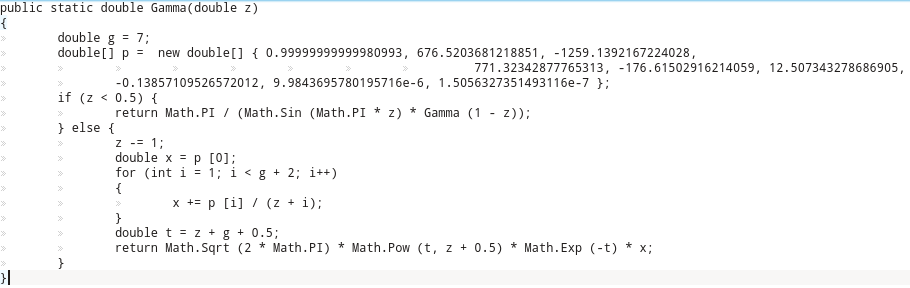
\includegraphics[scale=0.4]{code}
\end{figure}
\end{frame}

\begin{frame}{My Favourite Picture}
\begin{figure}[scale=0.5]
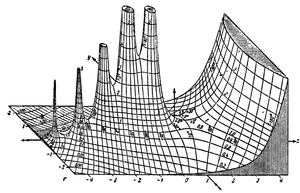
\includegraphics[scale=0.8]{Jahnke_gamma_function}
\caption{Hand drawn graph of the absolute value of the gamma function in the complex plane from \emph{Tables of Higher Functions} by Jahnke and Emde}
\end{figure}
\end{frame}
\end{document}
